%Arik Messerman, September 2006, uidarikmesserman301174 003 0021
%%% HAUPTTEIL ***

%%%%%%%%%%%%%%%%%%%%%%%%%%%%%%%%%%%%%%%%%%%%%%%%%%%%%%%%%%%%%%%%%%%%%%%%%%%%
% Pre�mbel
%%%%%%%%%%%%%%%%%%%%%%%%%%%%%%%%%%%%%%%%%%%%%%%%%%%%%%%%%%%%%%%%%%%%%%%%%%%%
\documentclass[12pt,a4paper,titlepage,oneside,BCOR1cm]{report}

\usepackage{ngerman} % neue deutsche Rechtschreibung
\usepackage[latin9]{inputenc} % latin9-Kodierung f�r Umlaute (Erweiterung von latin1)
\usepackage[T1]{fontenc} 
% Sprachen:
\usepackage[ngerman]{babel} % Silbentrennung Deutsch neue Rechtschreibung
\selectlanguage{ngerman}

\sloppy
\usepackage{amsmath,marvosym} % Mathematik
\usepackage{times}
\usepackage{setspace} % 1,5 Zeilenabstand
\onehalfspacing

% Literatur
\usepackage{bibgerm}
\pagestyle{headings}
\bibliographystyle{gerunsrt} % Literaturangaben nach Auftreten sortieren %{gerplain}
\usepackage{sty/abbreviations}

\usepackage{graphicx} % Bilder einf�gen
\usepackage{subfigure} % mehrere Abbildungen nebeneinander/�bereinander
% aller Bilder werden im Unterverzeichnis figures gesucht:
\graphicspath{{figures/}}
\usepackage{latexsym}

\usepackage{fancyhdr} %Kopf- und Fu�zeilen
\setcounter{secnumdepth}{4}
\setcounter{tocdepth}{3} 

% Hurenkinder- und Schusterjungenregelung
\clubpenalty = 10000 % schliesst Schusterjungen aus
\widowpenalty = 10000 % schliesst Hurenkinder aus

\pagestyle{fancy}
\pagestyle{headings}
\usepackage{url, geometry, amssymb, graphicx, booktabs}

% PDF
\usepackage[colorlinks,pagebackref,pdfpagelabels]{hyperref} %Hyperlinks zw. Textstellen
\usepackage[hyphenbreaks]{breakurl}
\usepackage{color} % Farben
\hypersetup{
frenchlinks=false,
colorlinks=false,
bookmarksopen=true,
bookmarksnumbered=true,
pdftitle = {Seminararbeit},
pdfsubject = {Seminararbeit},
pdfauthor = {Arik Messerman},
pdfkeywords = {uidarikmesserman301174 003 0021, arik messerman},
pdfcreator = {Adobe-Acrobat-Distiller},
pdfproducer = {LaTeX with hyperref and thumbpdf}
}

%%%%%%%%%%%%%%%%%%%%%%%%%%%%%%%%%%%%%%%%%%%%%%%%%%%%%%%%%%%%%%%%%%%%%%%%%%%%%%%%%%%%%%%%%%%%%%
% Hier bitte Werte �ndern %%%%%%%%%%%%%%%%%%%%%%%%%%%%%%%%%%%%%%%%%%%%%%%%%%%%%%%%%%%%%%%%%%%%
\date{September 2006}
\author{Arik Messerman}
\title{Dokumentenvorlage f�r eine Seminararbeit} % Bitte unter chapter/deckblatt.tex �ndern!!
%%%%%%%%%%%%%%%%%%%%%%%%%%%%%%%%%%%%%%%%%%%%%%%%%%%%%%%%%%%%%%%%%%%%%%%%%%%%%%%%%%%%%%%%%%%%%%

%%%%%%%%%%%%%%%%%%%%%%%%%%%%%%%%%%%%%%%%%%%%%%%%%%%%%%%%%%%%%%%%%%%%%%%%%%%%
% Beginn des Dokumentes
%%%%%%%%%%%%%%%%%%%%%%%%%%%%%%%%%%%%%%%%%%%%%%%%%%%%%%%%%%%%%%%%%%%%%%%%%%%%

\begin{document}
%\maketitle

\pagenumbering{Roman} % R�mische Aufz�hlung

%Arik Messerman, September 2006, uidarikmesserman301174 003 0021
%%% DECKBLATT ***

% Hier bitte nur ab markierten Bereich Daten �ndern

\thispagestyle{empty}
\begin{figure}[htbp]
	\centering
  \begin{minipage}[b]{41 mm}
    %
\includegraphics[width=40 mm]{AOT-Logo.png}  
    %\includegraphics[width=40 mm]{dai_logo_engl.png}
    \includegraphics[width=40 mm]{dai_logo.png}
  \end{minipage}
  %\begin{minipage}[b]{73 mm}
  % 
\includegraphics[width=72 mm]{figures/FakAOT2.png}  
  %\end{minipage}
	%\begin{minipage}[b]{30 mm}
  %  \includegraphics[width=30mm]{figures/TU2.png}  
  %\end{minipage}
  \label{Labelname}
\end{figure}


% Ab hier d�rfen �nderungen vorgenommen werden
\begin{center}
\begin{Huge}
Technische Universit�t Berlin\\
\vspace{1mm}
\end{Huge}{\Large Fakult�t IV - Elektrotechnik und Informatik\\
Fachgebiet AOT\\
Prof. Dr. Sahin Albayrak}\\

\vspace{26mm}
\begin{LARGE}
Dokumentenvorlage f�r einen Projektabschlussbericht\\
\end{LARGE}
\vspace{8mm}
Projekt\\
\large Sicherheit in Verteilten Umgebungen\\
\normalsize Wintersemester 2006/07\\
\vspace{4 cm}
Arik Messerman \\
Matrikel--Nummer 123456\\
\vspace{1cm}
\begin{tabular}{ll}
{\bf Betreuer} & Max Musterbetreuermann\\
\end{tabular}

\end{center}
\clearpage

 % Titelseite
\clearpage
\chapter*{ }
\clearpage


\addcontentsline{toc}{chapter}{\numberline{}\contentsname} % Auch Inhaltsverzeichnis aufnehmen
\tableofcontents % Inhaltsverzeichnis
\clearpage

\addcontentsline{toc}{chapter}{\numberline{}\listfigurename} % Auch Abbildungsverzeichnis aufnehmen
\listoffigures % Abbildungsverzeichnis
\clearpage

% Tabellenverzeichnis
\addcontentsline{toc}{chapter}{\numberline{}\listtablename} % Auch Tabellenverzeichnis aufnehmen
\listoftables 
\newpage

%%%%%%%%%%%%%%%%%%%%%%%%%%%%%%%%%%%%%%%%%%%%%%%%%%%%%%%%%%%%%%%%%%%%%%%%%%%%%%%%%%%%%%%%%%%%%%

% Merke die r�mische Seitenzahl in 'roemisch'
\newcounter{roemisch}
\setcounter{roemisch}{\value{page}}
\pagenumbering{arabic}
\renewcommand{\chaptermark}[1]{\markboth{#1}{}}
\renewcommand{\sectionmark}[1]{\markright{\thesection\ #1}{}}
\fancyhead[LO]{}
\fancyhead[RO]{\slshape \rightmark}





%%%%%%%%%%%%%%%%%%%%%%%%%%%%%%%%%%%%%%%%%%%%%%%%%%%%%%%%%%%%%%%%%%%%%%%%%%%%
% Hauptteil (hier �nderungen vornehmen)
%%%%%%%%%%%%%%%%%%%%%%%%%%%%%%%%%%%%%%%%%%%%%%%%%%%%%%%%%%%%%%%%%%%%%%%%%%%%
\phantomsection
%Arik Messerman, September 2006, uidarikmesserman301174 003 0021
%%% KAPITEL 2 ***

\addcontentsline{toc}{chapter}{Hinweise}
\chapter*{Hinweise 1}

%\chapter{Hinweise} \label{kap2}
\section{Verzeichnisse und Nummerierung}
Hier ein kleiner Abschnitt zum Thema Nummerierung von Seitenzahlen, Abbildungen und Tabellen.
\subsection{Seitenzahlen}
Alle Seiten der Arbeit au�er der Titelseite sollten mit einer Seitenzahl versehen sein. Vor dem Beginn des ersten Kapitels werden im Allgemeinen r�mische Ziffern (i, ii, iii, iv, \dots) verwendet. Ab der ersten Seite des ersten Kapitels beginnt die Seitennummerierung neu und l�uft dann bis zur letzten Seite des Dokuments -- einschlie�lich Literaturverzeichnis und eventueller Anh�nge. Daf�r werden dann arabische Ziffern (1, 2, \dots) verwendet. 

\subsection{Abbildungen und Tabellen}
S�mtliche Abbildungen und Tabellen werden durchg�ngig in Abh�ngigkeit der Kapitelnummer nummeriert. Die Nummerierung lautet f�r Abbildungen z. B. \textit{``Abbildung~1.3''}, f�r Tabellen \textit{``Tabelle~2.2''}. Als Beispiele siehe Tabelle \ref{tab:EineTabelle} auf Seite \pageref{tab:EineTabelle} und Abbildung \ref{fig:agent} auf Seite \pageref{fig:agent}.
\begin{figure}[htb]
	\centering
		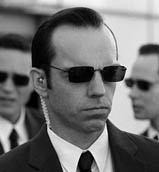
\includegraphics{figures/agent.jpg}
	\caption{Ein Agent}
	\label{fig:agent}
\end{figure}
Auf alle vorkommenden Abbildung und Tabellen muss im Text verwiesen werden. Ist der Inhalt nicht selbsterkl�rend, so sollte auch eine Erl�uterung gegeben werden. \\
Abbildungen oder Tabellen, die gr��er als etwa eine Drittel Seite sind, passen meist besser in den Anhang als in den laufenden Text. 
\begin{table}[ht]
	\centering
\begin{tabular}{||l|r|r|r|r||}
\hline
Verlauf &       2004 &       2005 &       2006 &       2007 \\
\hline
\hline
Deutschland &       2500 &          0 &       5000 &       4500 \\
\hline
   Italien &       1700 &       1000 &       3600 &       5000 \\
\hline
   Schweiz &       2000 &       2000 &       1500 &       2000 \\
\hline
\end{tabular}  

	\caption{Eine Tabelle}
	\label{tab:EineTabelle}
\end{table}
\\
Unter \cite{jam} kann man sich eines Freeware-Tools bedienen, welches die Erzeugung geeigneter \LaTeX -Codes ausgehend aus einer \emph{EXCEL}-Tabelle aus generiert.
\subsection{Inhaltsverzeichnis}
\LaTeX{} erstellt das Inhaltsverzeichnis automatisch aus den Formatvorlagen f�r die verschiedenen �berschriften. Unter Umst�nden ist eine mehrmalige �bersetzung erforderlich damit die Seitenzahlen �bereinstimmen. 

\subsection{Abbildungs- und Tabellenverzeichnis}
L�ngere wissenschaftliche Arbeiten enthalten normalerweise ein Abbildungs- und ein Tabellenverzeichnis. Im Rahmen einer kurzen Seminararbeit kann darauf verzichtet werden.

\section{Fu�noten}
Fu�noten\footnote{Dies ist die eine Fu�note} sollten nur sehr, sehr sparsam verwendet werden. Wenn die amerikanische Zitierweise verwendet wird, die bei der Themenvorstellung erl�utert wurde, kann man eigentlich ganz auf sie verzichten. Wenn unbedingt Fu�noten eingesetzt werden sollen, dann werden sie stets f�r je einen Kapitel fortlaufend mit arabischen Ziffern (1, 2, \dots) nummeriert\footnote{Dies ist weitere Fu�note}.

\section{Literatur und Zitate}
S�mtliche �bernommenen Ideen, Gedankeng�nge oder Formulierung von anderen Autoren m�ssen als Zitate gekennzeichnet werden und eine Quellenangabe gemacht werden. Enth�lt eine Arbeit nicht gekennzeichnete Zitate, so ist sie ein \textbf{Plagiat}. \\
Ins Literaturverzeichnis werden s�mtliche zitierten Quellen aufgenommen. Es werden keine Ver�ffentlichungen angef�hrt, die nicht in der Arbeit verwendet wurden. F�r weitere Hinweise siehe die Pr�sentationsfolien aus der Einf�hrungsveranstaltung.


\section{Layout}
Hier noch die wichtigsten Layout-Parameter:\\
\\
\begin{table}[ht]
	\centering
\begin{tabular}{|l|l|}
\hline
Schriftart/-gr��e: & Times/12pt \\
\hline
Seitenr�nder (oben/unten/innen/au�en): & 2,5/2,0/3,0/2,8 cm \\
\hline
Zeilenabstand: &    Einfach \\
\hline
Absatzabstand: &        6pt \\
\hline
\end{tabular}  
	\caption{Layout-Parameter}
	\label{tab:layout}
\end{table}
\\
\phantomsection
%Arik Messerman, September 2006, uidarikmesserman301174 003 0021
%%% KAPITEL 3 ***
\addcontentsline{toc}{chapter}{Hinweise 2}
\chapter*{Hinweise 2}

\section{Test des Layouts} \label{kap3}
Um die Lesbarkeit zu erleichtern ist es ratsam jedes Kapitel mit Worten einzuleiten, die beschreiben was man gleich lesen wird. Einleitende Worte und ein kurzer Abriss worauf man mit der Wahl der Unterkapitel abzielt \dots

\section{Erste Betrachtungen}
Bevor wir uns mit Details besch�ftigen erstmal \dots
\subsection{Ganzheitliche Analyse}
Am Tag nach der unerwarteten Arbeitszeitverl�ngerung verbarg Stevens seine pers�nlichen Gef�hle. Fragen zum Kampf um seinen Arbeitsplatz bei Hertha BSC wollte der Niederl�nder nicht mehr h�ren. ,,�ber meine Person spreche ich nicht mehr, da ist alles gesagt worden'', sagte Stevens vier Tage vor dem ersten seiner beiden pers�nlichen Entscheidungsspiele gegen Hansa Rostock. Nur mit Siegen am Samstag in der Bundesliga und am kommenden Dienstag im DFB-Pokal kann der 49 Jahre alte Trainer seinen Job in Berlin retten.\\

Unter einem grauen Berliner Himmel schien nach dem Ultimatum vom Montag der Alltag auf dem Trainingsplatz eingekehrt zu sein. Erst nach der ersten von zwei �bungseinheiten machte die Zur�ckhaltung der Hertha-Profis den Ernst der Lage beim �berraschenden Tabellenletzten wieder klar. ,,Wir wollen diese Woche in Ruhe arbeiten. Das hat die Mannschaft so vereinbart, das ist keine Anweisung von oben'', betonte Nationalspieler Marko Rehmer im Namen seiner Kollegen. Der Mannschaftsrat hatte in einer Erkl�rung mitgeteilt, er trage die ungew�hnliche Vereinbarung mit Stevens mit. \\

Die �ffentlichkeit in der Hauptstadt reagierte auf die vorl�ufige Weiterbesch�ftigung von Stevens mit Unverst�ndnis. ,,Stevens f�r Stevens'', wunderte sich die ,,Berliner Zeitung'' am Dienstag. ,,Berlin unter Schock'', titelte die ,,BZ'', der ,,Berliner Kurier'' formulierte drastisch Richtung Hertha: ,,Hertha BSE - ihr seid doch irre!'' Die ,,Berliner Morgenpost'' schrieb: ,,Heldenmut oder Starrsinn -- Dieter Hoene� unter Druck.'' Und der ,,Tagesspiegel'' sprach von einer Stevens-Bilanz ,,schwach wie im Aufstiegsjahr''. Die ,,Galgenfrist'' (,,M�rkische Oderzeitung'') wertete ,,Bild'' als Votum gegen die Fan-Mehrheit. 


\subsection{Detaillierte Betrachtung des Sachverhalts}
Am Tag nach der unerwarteten Arbeitszeitverl�ngerung verbarg Stevens seine pers�nlichen Gef�hle. Fragen zum Kampf um seinen Arbeitsplatz bei Hertha BSC wollte der Niederl�nder nicht mehr h�ren. ,,�ber meine Person spreche ich nicht mehr, da ist alles gesagt worden'', sagte Stevens vier Tage vor dem ersten seiner beiden pers�nlichen Entscheidungsspiele gegen Hansa Rostock. Nur mit Siegen am Samstag in der Bundesliga und am kommenden Dienstag im DFB-Pokal kann der 49 Jahre alte Trainer seinen Job in Berlin retten.\\

Die �ffentlichkeit in der Hauptstadt reagierte auf die vorl�ufige Weiterbesch�ftigung von Stevens mit Unverst�ndnis. ,,Stevens f�r Stevens'', wunderte sich die ,,Berliner Zeitung'' am Dienstag. ,,Berlin unter Schock'', titelte die ,,BZ'', der ,,Berliner Kurier'' formulierte drastisch Richtung Hertha: ,,Hertha BSE - ihr seid doch irre!'' Die ,,Berliner Morgenpost'' schrieb: ,,Heldenmut oder Starrsinn -- Dieter Hoene� unter Druck.'' Und der ,,Tagesspiegel'' sprach von einer Stevens-Bilanz ,,schwach wie im Aufstiegsjahr''. Die ,,Galgenfrist'' (,,M�rkische Oderzeitung'') wertete ,,Bild'' als Votum gegen die Fan-Mehrheit. 


\phantomsection
%Arik Messerman, September 2006, uidarikmesserman301174 003 0021
%%% KAPITEL 5 ***
\addcontentsline{toc}{chapter}{Hinweise 3}
\chapter*{Hinweise 3}

\section{LaTeX} \label{kap5}
Hier noch mal einiges kurz zum Aufbau der Vorlage.
\section{Bilder und Tabellen}
Alle Bilder befinden sich im Unterordner \textit{figures}. Die typische Einbindung eines Bildes sieht wie folgt aus:\\
\begin{verbatim}
\begin{figure}[htb]
\centering

\includegraphics[width=0.5\textwidth]{figures/DAI.jpg}
\caption{Hier ist ein Bild}
\label{fig:dai}
\end{figure}
\end{verbatim}
\begin{figure}[htb]
\centering

\includegraphics[width=0.5\textwidth]{figures/DAI.jpg}
\caption{Hier ist ein Bild}
\label{fig:dai}
\end{figure}
Auf diese Art und Weise eingef�gte Bilder werden automatisch durch das Abbildungsverzeichnis referenziert. Analoges gilt auch f�r Tabellen:\\
\begin{verbatim}
\begin{table}[htb]
\centering
\begin{tabular}{r|rrr}

           &          A &          B &          C \\
\hline
         1 &         a1 &         b1 &         c1 \\

         2 &         a2 &         b2 &         c2 \\

         3 &         a3 &         b3 &         c3 \\

         4 &         a4 &         b4 &         c4 \\

\end{tabular}
\caption{Hier ist eine Tabelle}
\label{tab:NochEineTabelle}  
\end{table}
\end{verbatim}
\begin{table}[htb]
\centering
\begin{tabular}{r|rrr}

           &          A &          B &          C \\
\hline
         1 &         a1 &         b1 &         c1 \\

         2 &         a2 &         b2 &         c2 \\

         3 &         a3 &         b3 &         c3 \\

         4 &         a4 &         b4 &         c4 \\

\end{tabular}
\caption{Hier ist eine Tabelle}
\label{tab:NochEineTabelle}  
\end{table}




%Arik Messerman, September 2006, uidarikmesserman301174 003 0021
%%% EINLEITUNG ***

\chapter{Einleitung} \label{einl}
Dieses Dokument gibt einen Strukurierungsvorschlag zum Projektabschlussbericht. Der Umfang sollte 20-40 Seiten (10-15 Seiten pro Person) betragen.
\section{Motivation}
Warum sich mit dem aktuellen Problem besch�ftigen?

\section{Ansatz}
Wie sieht die L�sung aus?

\section{Struktur}
Wie ist dieses Dokument aufgebaut?








\chapter{Problemanalyse}

Problemdarstellung
\chapter{L�sung}
Die umgesetzte L�sung

\section{Beschreibung L�sungsteil 1}
z.B. der Systemaufbau
\section{Beschreibung L�sungsteil 2}
z.B. das Interface
\section{Beschreibung L�sungsteil 3}
z.B. die Algorithmen

\chapter{Evaluierung}
Was bringt meine L�sung? Ist sie besser als andere?
%Arik Messerman, September 2006, uidarikmesserman301174 003 0021
%%% KAPITEL 4 ***

\chapter{Fazit und Ausblick} \label{kap4}
Welche Ergebnisse wurden erzielt? Welche Fragen sind offen geblieben? An welchen Punkten k�nnte in Zukunft weiter geforscht werden? Wie lassen sich theoretische Ergebnisse m�glicherweise in die Praxis umsetzen? Etc. (Maximal \(1\frac{1}{2}\)~Seiten).


\clearpage
%%%%%%%%%%%%%%%%%%%%%%%%%%%%%%%%%%%%%%%%%%%%%%%%%%%%%%%%%%%%%%%%%%%%%%%%%%%%
% Ende Hauptteil-
%%%%%%%%%%%%%%%%%%%%%%%%%%%%%%%%%%%%%%%%%%%%%%%%%%%%%%%%%%%%%%%%%%%%%%%%%%%%
	
% Setze Numerierung wieder auf r�misch zur�ck und setzte von oben fort
% Wert ist demnach der von 'roemisch'
%\pagenumbering{Roman}
%\setcounter{page}{\value{roemisch}}

%%%%%%%%%%%%%%%%%%%%%%%%%%%%%%%%%%%%%%%%%%%%%%%%%%%%%%%%%%%%%%%%%%%%%%%%%%%%
% Referenzen
%%%%%%%%%%%%%%%%%%%%%%%%%%%%%%%%%%%%%%%%%%%%%%%%%%%%%%%%%%%%%%%%%%%%%%%%%%%%
\addcontentsline{toc}{chapter}{\numberline{}\bibname}
\bibliography{chapter/bibliography} % Literaturverzeichnis



\appendix % andere Aufz�hlung
\clearpage

%%%%%%%%%%%%%%%%%%%%%%%%%%%%%%%%%%%%%%%%%%%%%%%%%%%%%%%%%%%%%%%%%%%%%%%%%%%%%%%%%%%%%%%%%%%%%%
% Hier kommen die Anh�nge %%%%%%%%%%%%%%%%%%%%%%%%%%%%%%%%%%%%%%%%%%%%%%%%%%%%%%%%%%%%%%%%%%%%
%Arik Messerman, September 2006, uidarikmesserman301174 003 0021
%%% ANHANG A ***

\chapter{Anhang -- Wenn ben�tigt} \label{anhA}
Falls kein Anhang ben�tigt wird, dann diese Seite(n) einfach l�schen.\\ 
Zum Beispiel f�r \\
Quellcode o. �.


\chapter{Abk�rzungsverzeichnis}

\begin{abbreviations}

% Bitte selbst alphabetisch sortieren !!!!!

\abbrev*{ieee}{IEEE}{Institute of Electrical and Electronics Engineers}
\abbrev*{lan}{LAN}{Local Area Network}
\abbrev*{wlan}{WLAN}{Wireless Local etwork Area}















\end{abbreviations}


\end{document}

